\section{Representative Examples}

Given the theoretical framework for downfolding a many-orbital (or many electron) problem to a 
few orbital (or few electron) problem, we now discuss examples which elucidate the 
AIDMD method. 
%The first example is mostly pedagogical, 
%where we have completely avoided the \textit{ab-initio} related complications of AIDMD. Rather, we use information directly available 
%from \textit{exact} eigenstates themselves to downfold from a lattice model with more orbitals (3-band model) 
%to one with fewer orbitals (1-band model). We then gradually increase the complexity of the problems we address 
%by downfolding the hydrogen chain in one dimension (with up to 10 atoms) and graphene 
%(with up to 32 carbons on a 2D honeycomb lattice). Finally, we use the matching pursuit algorithm discussed 
%in section 2, suited for multiple energy scales, for the case of transition metals 
%by considering the diatomic FeSe molecule.
%\lucas{What about this? } \HJC{Yes, this is good} 
The examples are as follows:
\begin{itemize}
\item Section~\ref{subsection:3band}: Three band Hubbard $\rightarrow$ one band Hubbard at half filling. Demonstrates finding a basis set for the second quantized operators and uses a set of eigenstates directly sampled from the low-energy space to find a one-band model.
\item Section~\ref{subsection:1dhydrogen}: Hydrogen chain $\rightarrow$ one band Hubbard model at half filling. Demonstrates basis sets for {\it ab-initio} systems and the possibility to use this technique to determine the quality of a model to a given physical situation.
\item Section~\ref{subsection:graphene}: Graphene $\rightarrow$ one band Hubbard model with and without $\sigma$ electrons. Demonstrates using the downfolding procedure to examine the effects of screening due to core electrons. 
\item Section~\ref{subsection:fese}: FeSe molecule $\rightarrow$ $d,p,4s$ system. Demonstrates the use of matching pursuit to assess the importance of terms in an effective model and to select compact effective models.
\end{itemize}

%\HJC{Lucas, Is this better?} \lucas{It still looks to me that this really goes in the 3-band part?} 
%\HJC{1-band comes in several subsections, hence the need to define it early?}
In all examples we will highlight the important ingredients associated with AIDMD. First and foremost, is the choice 
of low energy space or energy window i.e. how our database of wavefunctions was generated. Associated with this is 
the choice of the one body space in terms of which the effective Hamiltonian is expressed. Finally, we discuss 
aspects of the functional forms or parameterizations that are expected to describe our physical 
problem. An important effective Hamiltonian that enters three out of our four representative examples is 
the single (or 1-) band Hubbard model,
\begin{equation}
	\tilde{H} = -t \;\sum_{\langle i,j \rangle} \tilde{d}_i^{\dagger} \tilde{d}_j + U \;\sum_{i} \tilde{n}^{i}_{\uparrow} \tilde{n}^{i}_{\downarrow}
\label{eq:oneband}
\end{equation}
where $t$ and $U$ correspond to downfolded (renormalized) parameters and $\tilde{d}$ are the effective one-particle operators. 
%which are obtained from transformations on their bare counterparts. 
%Thus %the determination of effective Hamiltonians is a \emph{dual} problem - what are the composite objects ($\tilde{d}_i$ here) 
%that give a compact description of the low energy physics? and given this choice what 
%are the effective interactions between them?

\subsection{Three-band Hubbard model to one band Hubbard model at half filling}
\label{subsection:3band} 
\HJC{Still editing - need to incorporate Lucas suggestions for energy dep..}
Our first example is motivated by the high $T_c$ superconducting cuprates~\cite{Bednorz1986} that 
have parent Mott insulators with rich phase diagrams on electron or hole doping~\cite{Dagotto_RevModPhys, LeeWen_RevModPhys}. 
Many works have been devoted to their model Hamiltonians and corresponding parameter 
values~\cite{Emery, ZhangRice, tJSpalek, Hybertsen_PRB1989, Hybertsen_PRB1990, Pavirini, Kent_Hubbard} and the 
emergent consensus of the minimal model involving both the copper and oxygen degrees of freedom 
is the 3-orbital or 3-band Hubbard model, 
\begin{eqnarray}
H &=&    \epsilon_p \sum_{j,\sigma} n^{p}_{j,\sigma} + \epsilon_{d} \sum_{i,\sigma}  n^{d}_{i,\sigma} 
	+ t_{pd} \sum_{\langle i,j \rangle, \sigma} \text{sgn}(p_i,d_j) \Big( d_{i,\sigma}^{\dagger} p_{j,\sigma} + \text{h.c.} \Big) \nonumber \\
  & &   + U_p \sum_{j} n^{p}_{j,\uparrow} n^{p}_{j,\downarrow} + U_d \sum_{i} n^{d}_{i,\uparrow} n^{d}_{i,\downarrow} + V_{pd} \sum_{\langle i,j \rangle} n^{j}_p n^{i}_d 
\end{eqnarray}
%\begin{eqnarray}
%H &=&    \epsilon_p \sum_{j,\sigma} n^{p}_{j,\sigma} + \epsilon_{d} \sum_{i,\sigma}  n^{d}_{i,\sigma} 
%	+ t_{pd} \sum_{\langle i,j \rangle, \sigma} \text{sgn}(p_i,d_j) \Big( d_{i,\sigma}^{\dagger} p_{j,\sigma} + \text{h.c.} \Big) + U_p \sum_{j} n^{p}_{j,\uparrow} n^{p}_{j,\downarrow} + U_d \sum_{i} n^{d}_{i,\uparrow} n^{d}_{i,\downarrow} + V_{pd} \sum_{\langle i,j \rangle} n^{j}_p n^{i}_d 
%\end{eqnarray}
where $d_i,p_j$ refer to the  $d_{x^2 - y^2}$ orbitals of copper (at site $i$) and $p_x$ or $p_y$ 
oxygen (at site $j$)  respectively and $\text{sgn}(p_i,d_j)$ is the sign of the hopping $t_{pd}$ 
between them, shown schematically in Fig.~\ref{fig:threeband}. 
$\epsilon_d$,$\epsilon_p$ are orbital energies, $U_d$, $U_p$ are strengths of onsite Hubbard interactions 
and $V_{pd}$ is the strength of the density-density interactions between a neighboring $p$ and $d$ orbital. 
We keep the exposition simple and consider only the case where $\epsilon_p$, $U_d$ and $t_{pd}$ 
are non zero; the latter is chosen throughout this section to be the typical value of $1.3$ eV to give the reader a sense of overall scale. 
Since we work with fixed number of particles we set our reference zero energy 
to be $\epsilon_d = 0$, thus the charge transfer energy $\Delta \equiv \epsilon_p - \epsilon_d$ equals $\epsilon_p$ in our notation. 
We work in the hole notation; half filling corresponds to 2$\uparrow$ and 2$\downarrow$ holes on the $2\times2$ cell.
\begin{figure}[htpb]
\centering

\includegraphics[width=0.8\linewidth]{./Figures/three_band_figure.eps}
\caption{Schematic for downfolding the three band Hubbard model to the one band Hubbard model. The oxygen orbitals are 
eliminated to give "dressed" $d$-like orbitals of the one band model, with modified hopping and interaction parameters. 
The relationship between the $\tilde{d}$ and the copper and oxygen orbitals is encoded by a linear transformation 
${\bf T}$ which is parameterized by $\alpha_1$, $\alpha_2$, $\alpha_3$, $\alpha_4$ and $F$ (see text for more details).}
\label{fig:threeband} 
\end{figure}

<<<<<<< HEAD
It is our objective to determine what 1-band Hubbard model ``best" describe the 3-band data, the former defined 
in terms of effective \textit{d-like} orbitals, $\tilde{d}$, which are mixtures (\HHZ{mixtures $\to$ hybridization?}) of copper and oxygen orbitals; 
this optimal transformation also remains an unknown. This is a \emph{dual} problem - what are the composite objects 
($\tilde{d}_i$ here) that give a compact description of the low energy physics? and given this choice what 
are the effective interactions between them?

In addition, the ``best" effective Hamiltonian description depends on the energy scale of interest. 
We first focus on the lowest scales and use our knowledge of the exact 
eigenstates of the 3-band and 1-band models to perform a state by state comparison. 
This is verified by the standard protocol (of section 2) in this energy window. Then, to build faith 
in the results, the predictions of the 1-band Hubbard parameters are tested on a larger cluster (8 unit cells). 
Finally, the standard protocol is used in a bigger energy window and it is shown that the optimal 
parameters are dependent on the energy window of interest. This exercise will serve 
as a guide for other sections. 
=======
It is our objective to determine what 1-band Hubbard model~(Eq.~\ref{eq:oneband}) 
"best" describe the 3-band data. The effective \textit{d-like} orbitals, $\tilde{d}$ entering the low energy description 
are mixtures of copper and oxygen orbitals; this optimal transformation also remains an unknown. 
Thus the model determination is a \emph{dual} problem (1) 
what are the composite objects that give a compact description of the low energy physics? and (2) 
given this choice what are the effective interactions between them? 
In addition, the "best" effective Hamiltonian description depends on the energy scale of interest. 
All these issues will be clarified in the remainder of the section. 
>>>>>>> 37b2347fa760c029d4d3358451cf81d6a0e94b1a

%We first focus on the lowest scales and use our knowledge of the exact 
%eigenstates of the 3-band and 1-band models to perform a state by state comparison. 
%This is verified by the standard protocol (of section 2) in this energy window. Then, to build faith 
%in the results, the predictions of the 1-band Hubbard parameters are tested on a larger cluster (8 unit cells). 
%Finally, the standard protocol is used in a bigger energy window and it is shown that the optimal 
%parameters are dependent on the energy window of interest. This exercise will serve 
%as a guide for other sections. 
We begin by encoding the relationship between the bare and effective operators as a linear transformation ${\bf T}$, 
\begin{equation}
	\tilde{d}_{i,\sigma} = \sum_{j} T_{ij} c_{j,\sigma}
\label{eq:dc}
\end{equation}
where $c_{j,\sigma}$ is the bare hole (destruction) operator and refers to either the bare $d$ or $p$ orbitals. 
Higher body generalizations are also possible, but have not been considered here. 
For the $2\times2$ unit cell, {\bf T} is a $4 \times 12 $ matrix, and accounting for its symmetries 
for the numbering of the orbitals corresponding to Fig.~\ref{fig:threeband}, it is explicitly written out as, 
\begin{eqnarray}
{\bf T} = 
\left(
\begin{array}{cccccccccccc}
F        & \alpha_2 &        \alpha_2 &  \alpha_4 & \alpha_1 & \alpha_1 & -\alpha_1 & -\alpha_1 & \alpha_3 & -\alpha_3 & \alpha_3 & -\alpha_3 \\
\alpha_2 &  F       &        \alpha_4 &  \alpha_2 & \alpha_3 & -\alpha_1 & \alpha_1 & -\alpha_3 & -\alpha_3 & \alpha_3 & \alpha_1 & -\alpha_1 \\
\alpha_2 & \alpha_4 & F               &  \alpha_2 & -\alpha_1 & \alpha_3 & -\alpha_3 & \alpha_1 & \alpha_1 & -\alpha_1 & -\alpha_3 & \alpha_3 \\
\alpha_4 & \alpha_2 & \alpha_2        &   F       & -\alpha_3 & -\alpha_3 & \alpha_3 & \alpha_3 & -\alpha_1 & \alpha_1 & -\alpha_1 & \alpha_1 \\
\end{array}
\right)
\end{eqnarray}
where we have defined $F \equiv \sqrt{1-4{\alpha_1}^2 - 2{\alpha_2}^2 - 4 {\alpha_3}^2 -{\alpha_4}^2}$ and 
where the parameters $\alpha_1$,$\alpha_2$,$\alpha_3$ and $\alpha_4$ will be optimized to minimize a 
certain cost function, which will be explained shortly. 

The density matrices in eigenstate $s$ in the transformed basis are related to that in the original basis by,
\begin{subequations}
\begin{eqnarray}
	\langle {\tilde{d}_{i,\sigma}}^{\dagger} \tilde{d}_{j,\sigma} \rangle_{s} &=& \sum_{mn} T^{*}_{im} \langle {c_{m,\sigma}}^{\dagger} c_{n,\sigma} \rangle_{s} T_{jn} \label{eq:dmstransformations1} \\
	\langle \tilde{n}_{i,\uparrow} \tilde{n}_{i,\downarrow} \rangle_{s} &=& \sum_{jkmn} T^{*}_{ij} T^{*}_{im} \langle {c_{j,\uparrow}}^{\dagger} {c_{m,\downarrow}}^{\dagger} c_{n,\downarrow} c_{k,\uparrow} \rangle_{s} T_{in} T_{ik}
\label{eq:dmstransformations2}
\end{eqnarray}
\end{subequations}
We optimize the transformation by demanding two conditions be satisfied, (1) the effective orbitals ($\tilde{d}_{i,\sigma}$) 
are orthogonal to each other i.e. $\Big({\bf T} {\bf T}^{\dagger}\Big)_{mn} = \delta_{mn}$
and (2) the sum of all diagonal entries (trace) of the 1-RDM of the effective orbitals for all low energy eigenstates 
equals the number of electrons of a given spin i.e. $\sum_{i} \sum_{\sigma} \langle {\tilde{d}_{i,\sigma}}^{\dagger} \tilde{d}_{i,\sigma} \rangle_{s} = N_{\sigma}$. 
These conditions are enforced by minimizing a cost function,
\begin{equation}
C = \sum_{s} \sum_{\sigma} \Big( \sum_{i} \langle \tilde{d}_{i,\sigma}^{\dagger} \tilde{d}_{i,\sigma} \rangle_{s} - N_{\sigma} \Big)^{2} + \sum_{mn} ( \Big({\bf T} {\bf T}^{\dagger}\Big)_{mn} -\delta_{mn})^{2}
\label{eq:C}
\end{equation} 

Fig.~\ref{fig:varyUdep} shows that in most regimes of the 3-band model, the lowest six eigenstates 
are separated from the higher energy manifold; we will show that they do 
correspond to states that can be described by the 1-body space of $\tilde{d}$ and hence can be described by a 1-band model. 
To give a concrete and representative example of our results, we discuss the case of 
$U_d/t_{pd}=8$ and $\Delta/t_{pd}=3$. Out of the lowest six, we chose only the lowest three eigenstates 
of the 3-band model for computing the cost in Eq.~\ref{eq:C} and found the optimal parameters of 
${\bf T}$ to be $\alpha_1=0.220$, $\alpha_2=0.044$, $\alpha_3=0.020$ and $\alpha_4=0.018$. 
The corresponding trace conditions and orthogonality are individually 
satisfied to a relative error of the order of 0.1 percent, verifying 
the validity of Eq.~\ref{eq:dc}.
% Get rid of this and possibly put in appendix
%\begin{small}
%\begin{eqnarray}
%\left(
%\begin{array}{cccc}
%+0.499 & -0.158 & -0.158 & 0.000  \\
%-0.158 & +0.499 &  0.000 & -0.158 \\
%-0.158 &  0.000 & +0.499 & -0.158 \\
% 0.000 & -0.158 & -0.158 & +0.499 \\
%\end{array}
%\right);
%\left(
%\begin{array}{cccc}
%+0.498 & -0.141 & -0.141 & -0.001  \\
%-0.141 & +0.498 & -0.001 & -0.141 \\
%-0.141 & -0.001 & +0.498 & -0.141 \\
%-0.001 & -0.141 & -0.141 & +0.498 \\
%\end{array}
%\right)
%;\left(
%\begin{array}{cccc}
%+0.498 & -0.083 & -0.083 & -0.032  \\
%-0.083 & +0.498 & -0.032 & -0.083 \\
%-0.083 & -0.032 & +0.498 & -0.083 \\
%-0.032 & -0.083 & -0.083 & +0.498 \\
%\end{array}
%\right)
%\end{eqnarray}
%\end{small}

Importantly, the 1-RDM elements corresponding to nearest neighbors $\langle \tilde{d}_1^{\dagger} \tilde{d}_2 \rangle_s$; 
already provide estimates for $U/t$ of the effective model. 
For our test example, in states 1, 2, and 3 their absolute values of $\langle \tilde{d}_1^{\dagger} \tilde{d}_2 \rangle_s$ 
are approximately $0.159$, $0.142$ and $0.084$ respectively. Since the exact knowledge of the 
corresponding eigenstates of the 1-band Hubbard model is directly available for arbitrary 
$U/t$ by numerical diagonalization, we directly look up the $U/t$ that would produce the same 1-RDM value.
This matching procedure gives $(U/t)_1 = $, $(U/t)_2$, $(U/t)_3 = $. Analogous estimates of $U/t$ were 
also made by comparing the 2-RDM elements $\langle \tilde{n}_{\uparrow} \tilde{n}_{\downarrow} \rangle_s$ 
with qualitatively similar results. 

This state-matching perspective was confirmed by performing the standard protocol (DMD) with the same three low-energy states, 
using their energies and the computed values of $\langle \tilde{d}_1^{\dagger} \tilde{d}_2 \rangle_s$ 
and $\langle \tilde{n}_{i,\uparrow} \tilde{n}_{i,\downarrow} \rangle_{s}$ from Eqs.~\eqref{eq:dmstransformations1} 
and~\eqref{eq:dmstransformations2}. 
(To mimic the situation characteristic of \textit{ab-initio} examples where no eigenstates are generally available, 
several non eigenstates were generated as random linear combinations of the lowest three eigenstates, with 
similar outcomes.) For our test example, this procedure provides an estimate of $U/t = $ and $t = $. 
As was expected, and observed, when the 1-band description is good, all estimates of $U/t$ 
%(be it from state by state comparison or the standard protocol) 
essentially agree with each other. 

%\begin{figure}[]
%\centering
%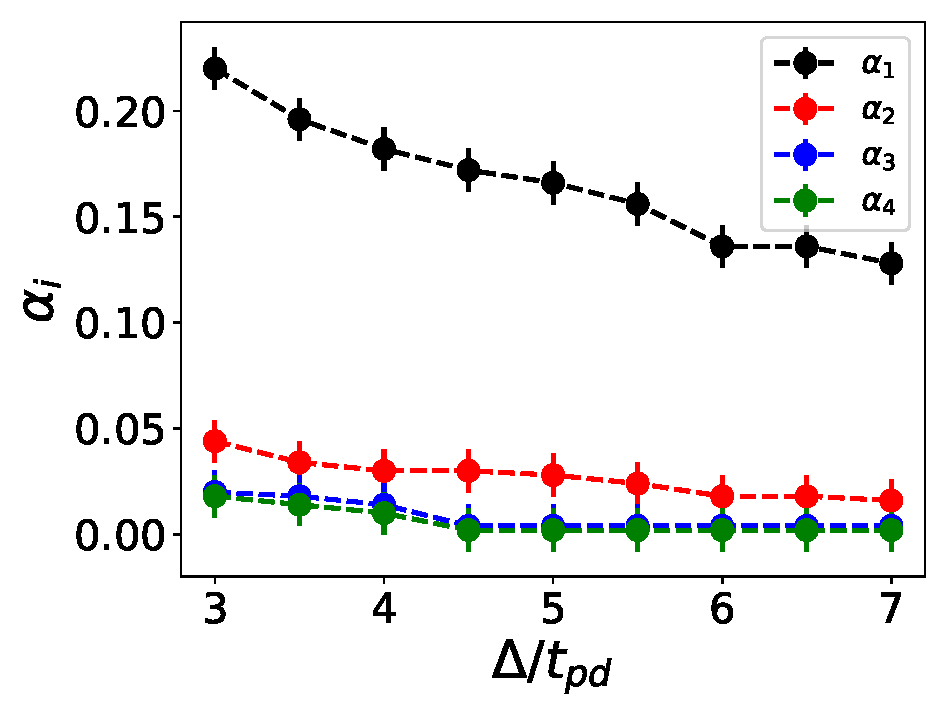
\includegraphics[width=0.49\linewidth]{./Figures/Hyb_vs_ep_Ud_8.pdf}
%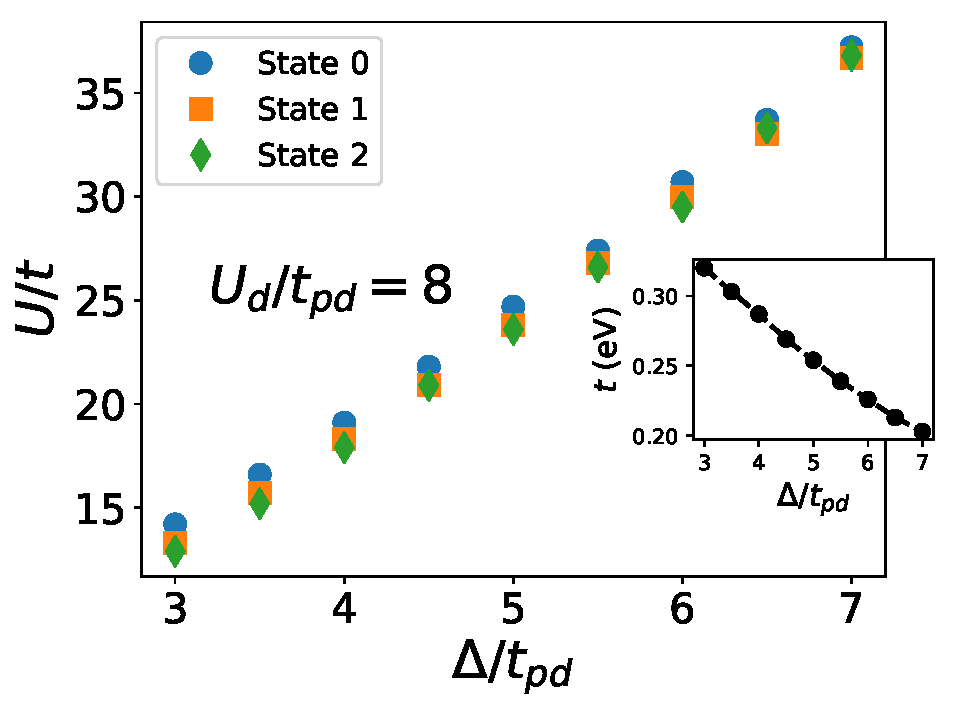
\includegraphics[width=0.49\linewidth]{./Figures/U_and_hopping_combined_vs_ep_Ud_8.pdf}
%\caption{(Left) Optimized values of parameters entering the transformation matrix 
%($\alpha_1$ through $\alpha_4$) and (Right) Effective 1-band Hubbard $U/t$ and hopping $t$ (inset) 
%versus $\Delta/t_{pd}$ for fixed $U_{d}/t_{pd}=8$}
%\label{fig:hamfitepdvary} 
%\end{figure}	
\begin{figure}[]
\centering
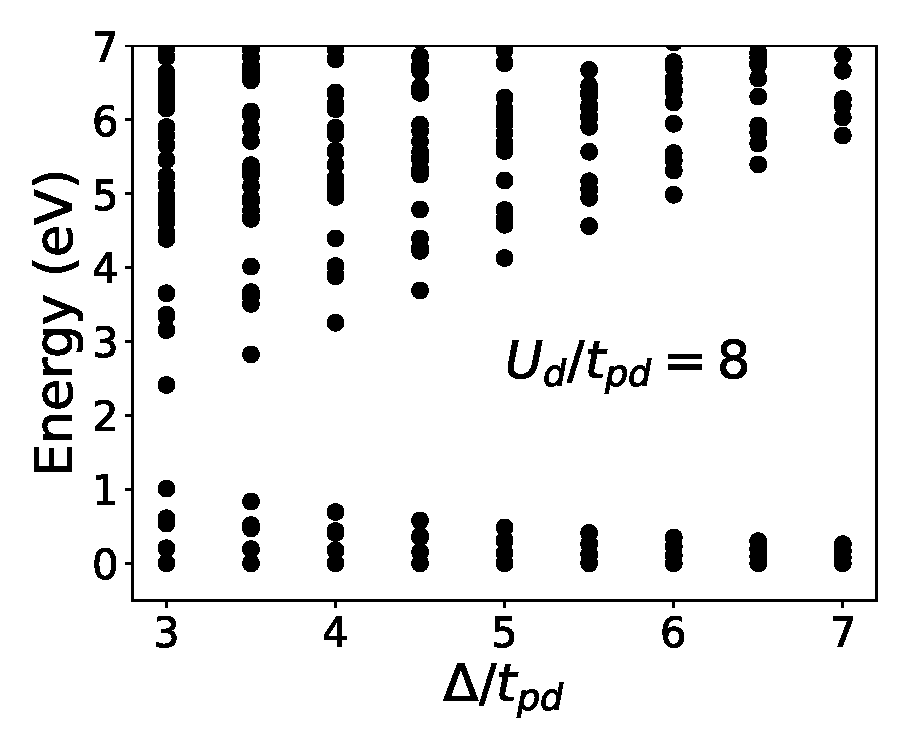
\includegraphics[width=0.45\linewidth]{./Figures/spectrum_vs_ep_Ud_8.eps}
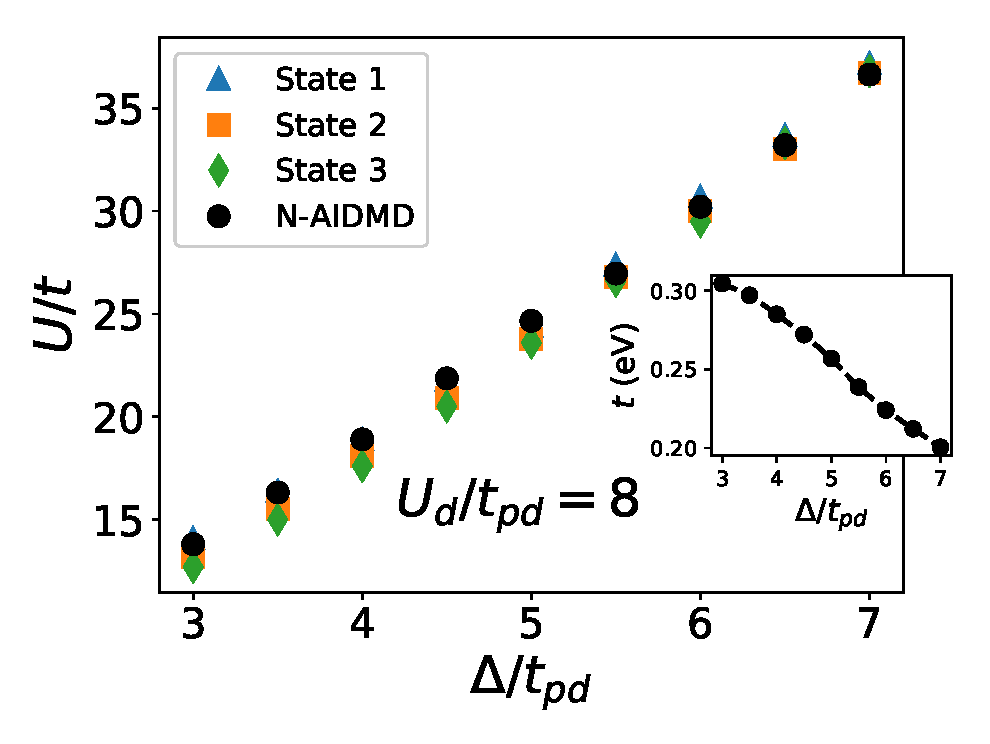
\includegraphics[width=0.49\linewidth]{./Figures/U_and_hopping_combined_vs_ep_Ud_8.eps}
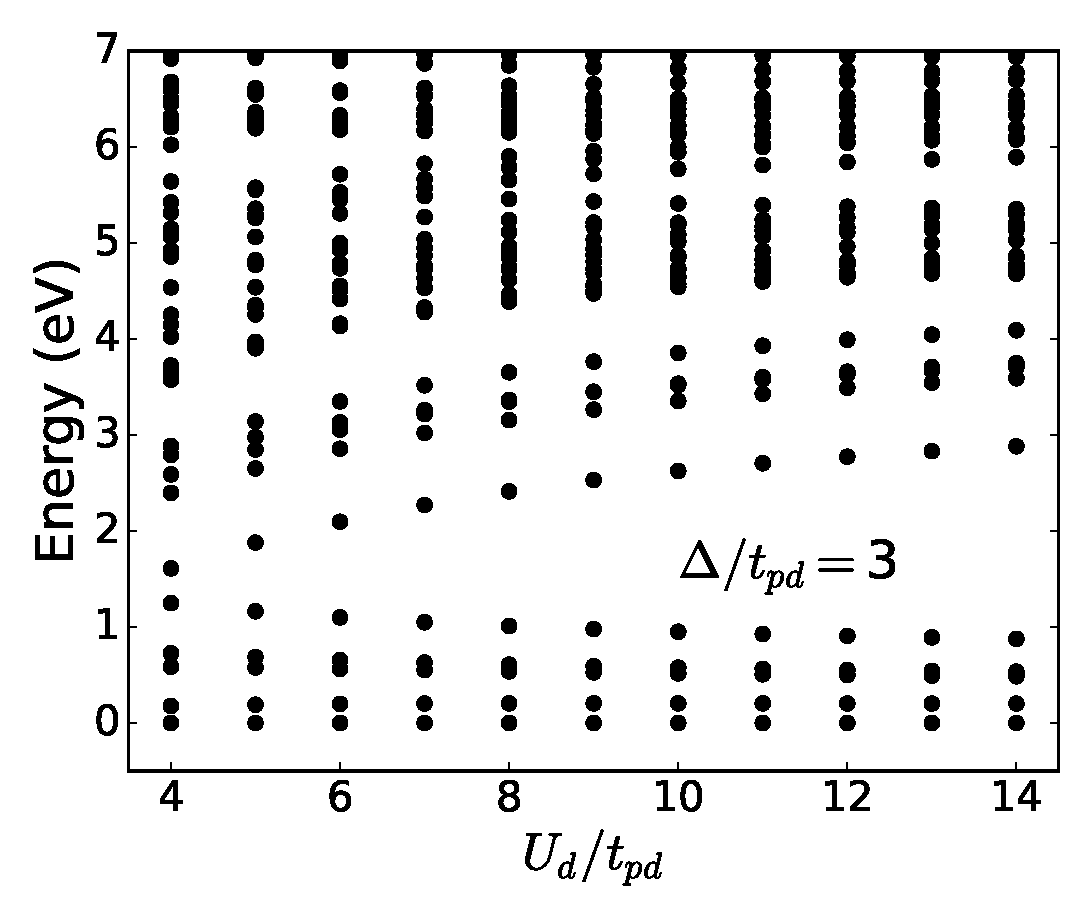
\includegraphics[width=0.45\linewidth]{./Figures/spectrum_vs_Ud_ep_3.eps}
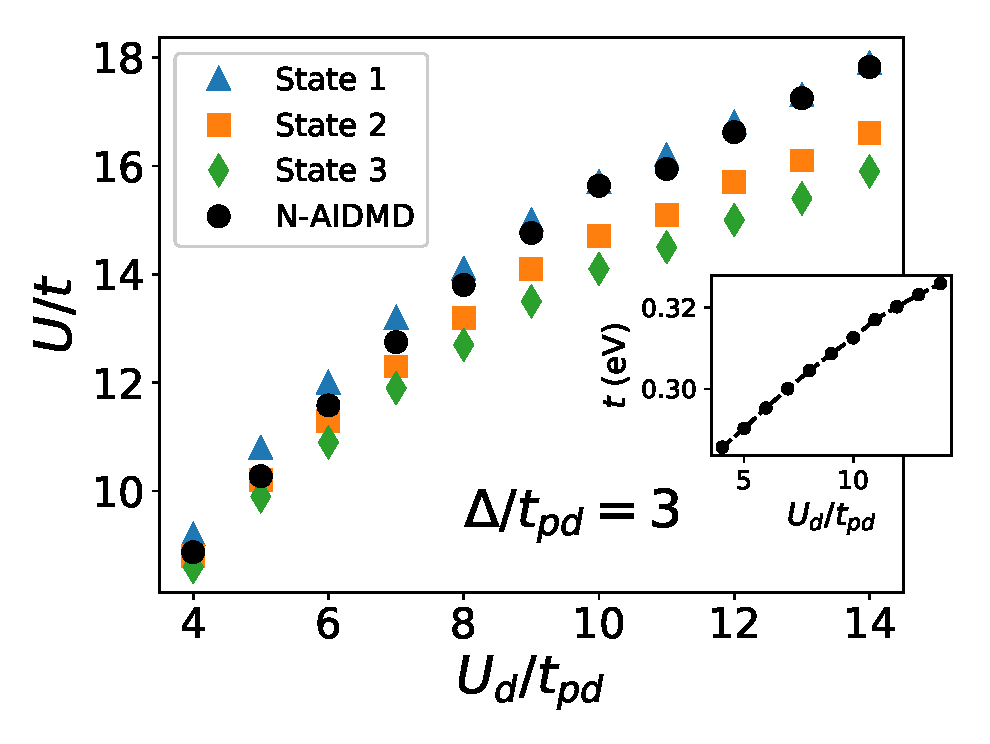
\includegraphics[width=0.48\linewidth]{./Figures/U_and_hopping_combined_vs_Ud_ep_3.eps}
%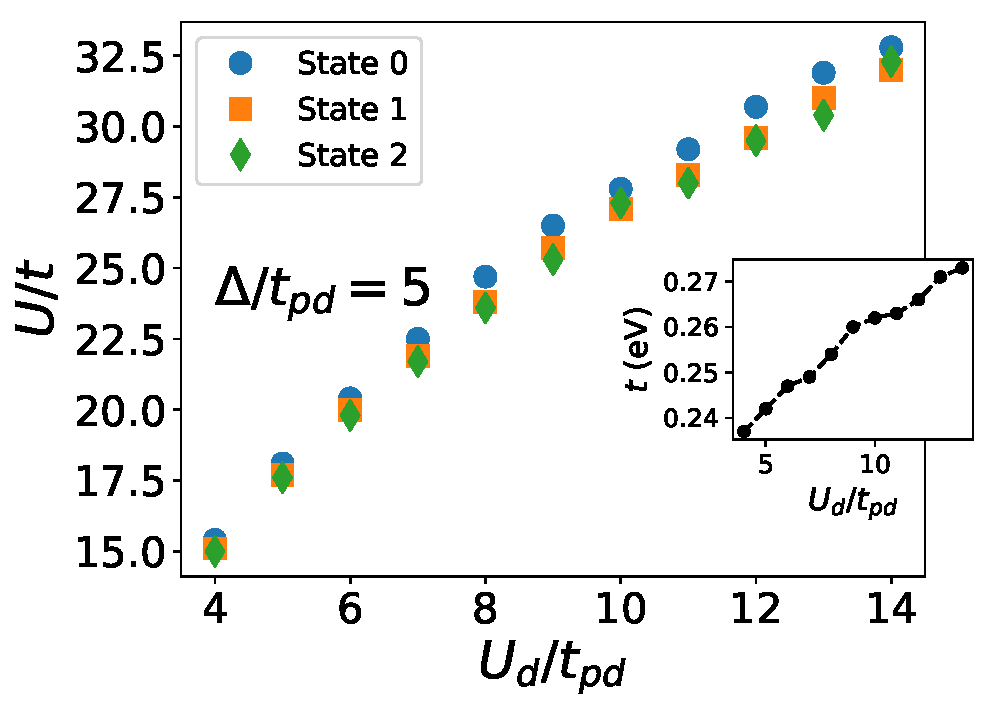
\includegraphics[width=0.50\linewidth]{./Figures/U_and_hopping_combined_vs_Ud_ep_5.pdf}
\caption{Low energy spectra (relative to the corresponding ground state) 
and estimates of downfolded parameters of the 1-band model for various parameter regimes of the 3-band Hubbard model. 
The estimates of $U/t$ were obtained by state matching or by the DMD procedure using 
the lowest three eigenstates. The top panels show the case of fixed $U_d/t_{pd}=8$ and varying $\Delta/t_{pd}$ 
and the bottom panels show the case of fixed $\Delta/t_{pd}=3$ and varying $U_d/t_{pd}$.}
\label{fig:varyUdep} 
\end{figure}	
 
Some trends in the 1-band description are explored in Fig.~\ref{fig:varyUdep} 
by monitoring the downfolded parameters as a function of varying $\Delta/t_{pd}$ and $U_d/t_{pd}$. 
For example, when $U_d/t_{pd}=8$ is fixed and $\Delta/t_{pd}$ is increased, we find that both 
the effective hopping in the 1-band model and the hybridization between nearest neighbor copper and oxygen $\alpha_1$ 
reduce and $U/t$ increases. This is physically reasonable since an increasing difference in the 
single particle energies of the copper and oxygen orbitals means the increased unfavorableness of holes 
to occupy the latter. When $\Delta/t_{pd}=3$ is fixed and $U_d/t_{pd}$ is increased, $U/t$ increases. 
As a way of avoiding the large $U_d$, the copper orbitals are forced to hybridize more with the oxygen ones; 
on the other hand the delocalization is suppressed in a bid to maintain mostly 
one electron per $\tilde{d}$ due to the larger $U/t$. 
The net result of these effects is that the effective $t$ also increases, albeit only marginally; a trend also observed in $\alpha_1$.

Since the standard protocol uses only information from the full (here, 3-band) model, it is imperative we 
perform other sanity checks on the accuracy of the downfolded model. An important check for the 1-band model is its 
ability to reproduce the low energy eigenenergies of the 3-band model. 
Fig.~\ref{fig:energyfit} shows the comparison of the energy gaps of the 
lowest six eigenstates of the 1-band and 3-band models. These six states correspond 
to 4C2 states of the effective spin model in its $S_z=0$ sector, all of which correspond to \textit{d like} spin excitations. 
The eigenstates above this manifold involve \textit{p-like} excitations, an aspect the 1-band model is not designed to capture. 
In all cases, the fit is reasonably good from an energetic viewpoint. 
%the best fits seen at larger $U_d$ and larger $\Delta$ consistent with our expectations from the previous plots. 
However, we also caution that the energy is relatively insensitive to small RDM elements, 
and that the Hubbard parameters can be strongly dependent on the energy window of interest, a point 
we highlight shortly. 
\begin{figure}[]
\centering
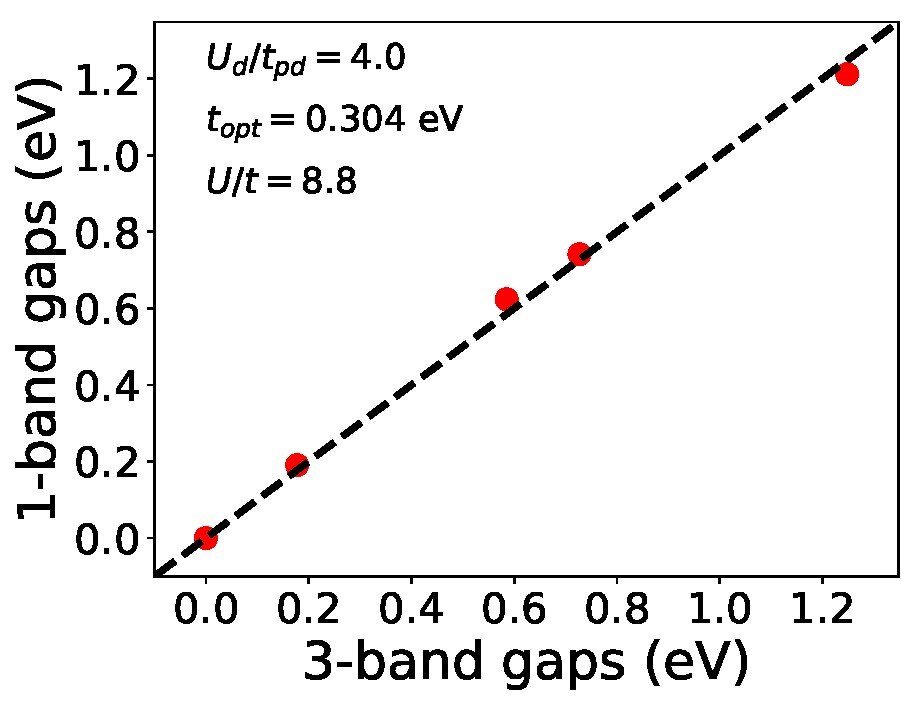
\includegraphics[width=0.325\linewidth]{./Figures/Gap_1_band_3_band_ep_3_number_5.pdf}
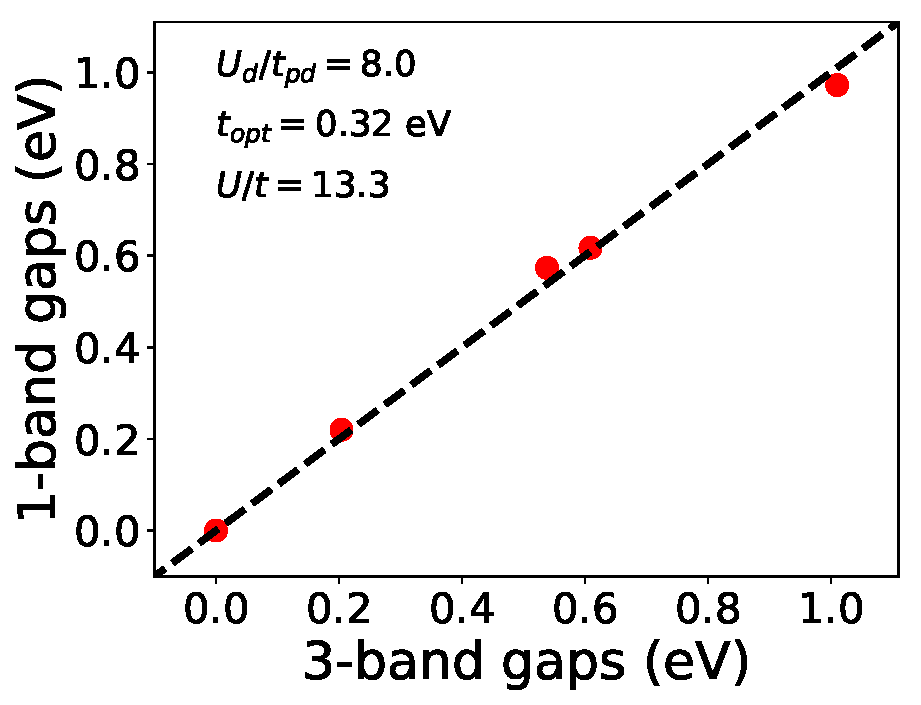
\includegraphics[width=0.325\linewidth]{./Figures/Gap_1_band_3_band_ep_3_number_9.pdf}
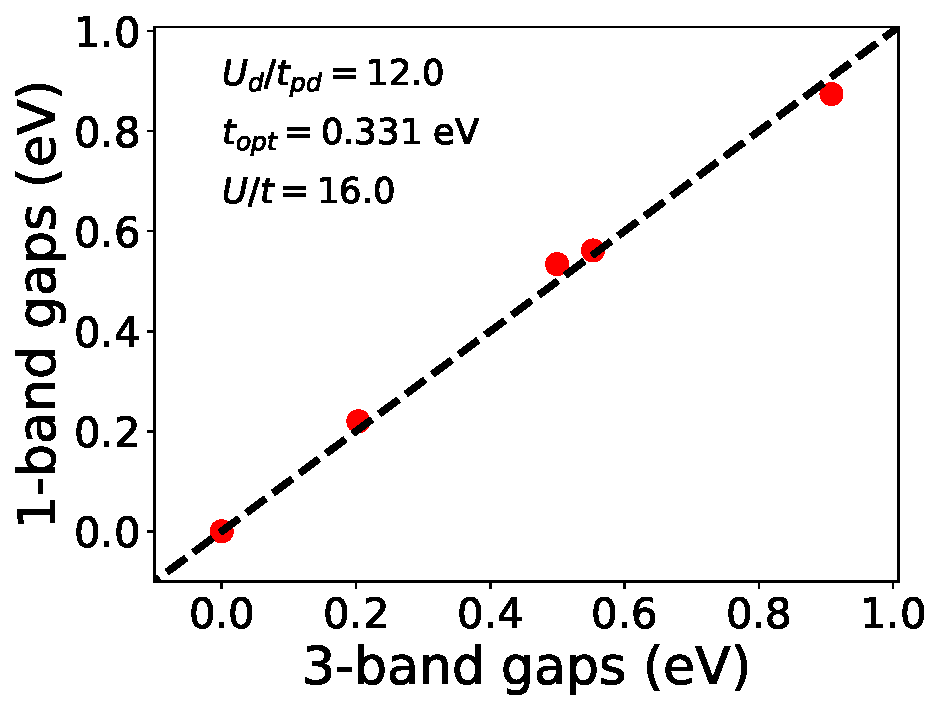
\includegraphics[width=0.325\linewidth]{./Figures/Gap_1_band_3_band_ep_3_number_2.pdf}
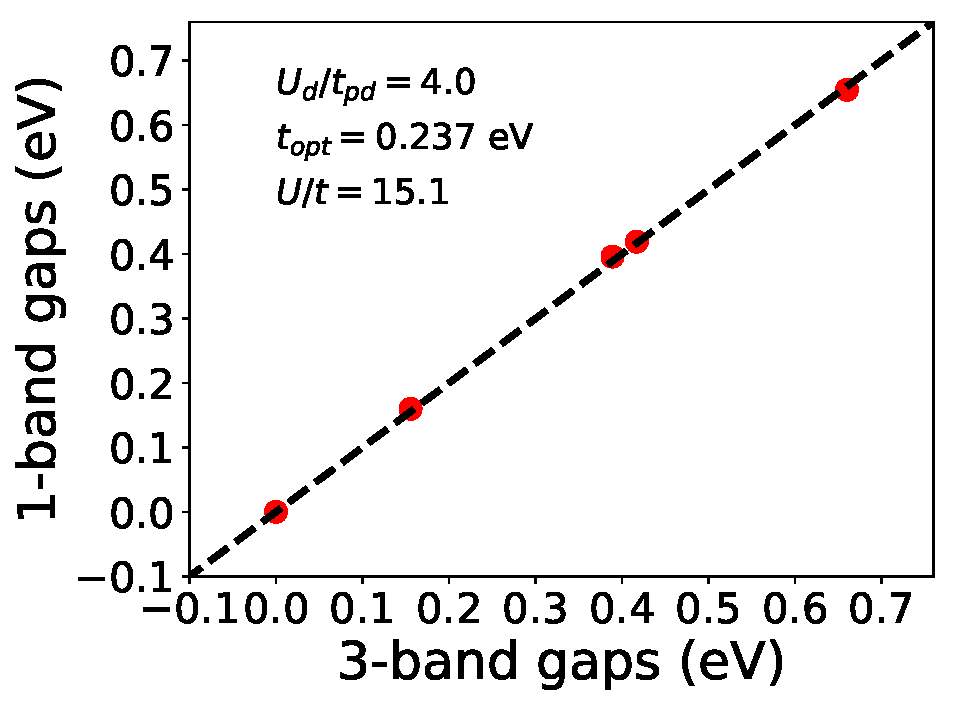
\includegraphics[width=0.325\linewidth]{./Figures/Gap_1_band_3_band_ep_5_number_5.pdf}
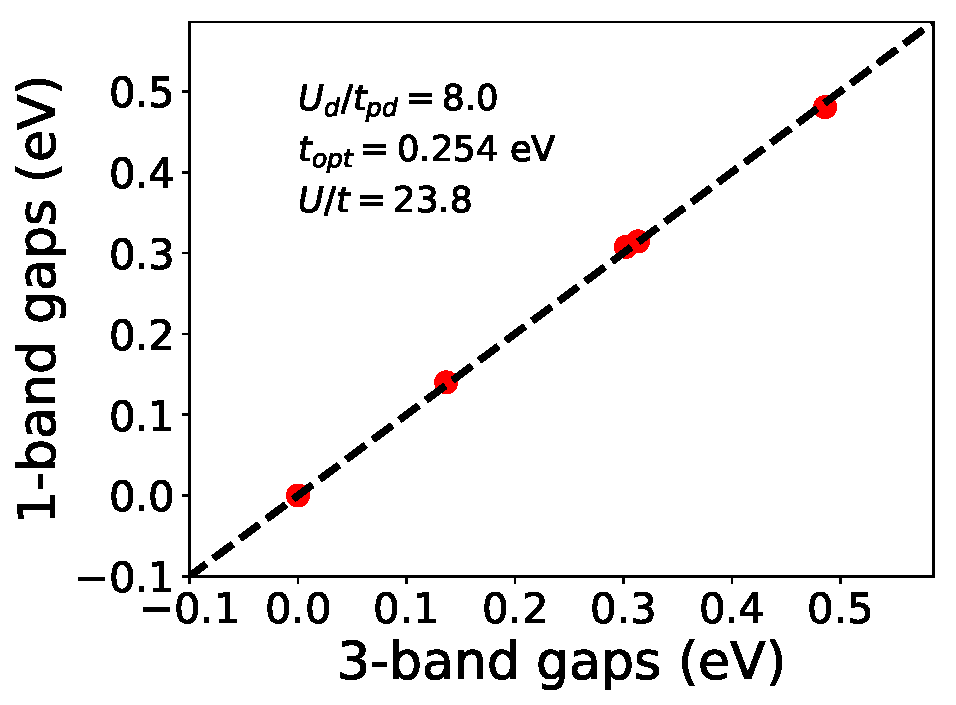
\includegraphics[width=0.325\linewidth]{./Figures/Gap_1_band_3_band_ep_5_number_9.pdf}
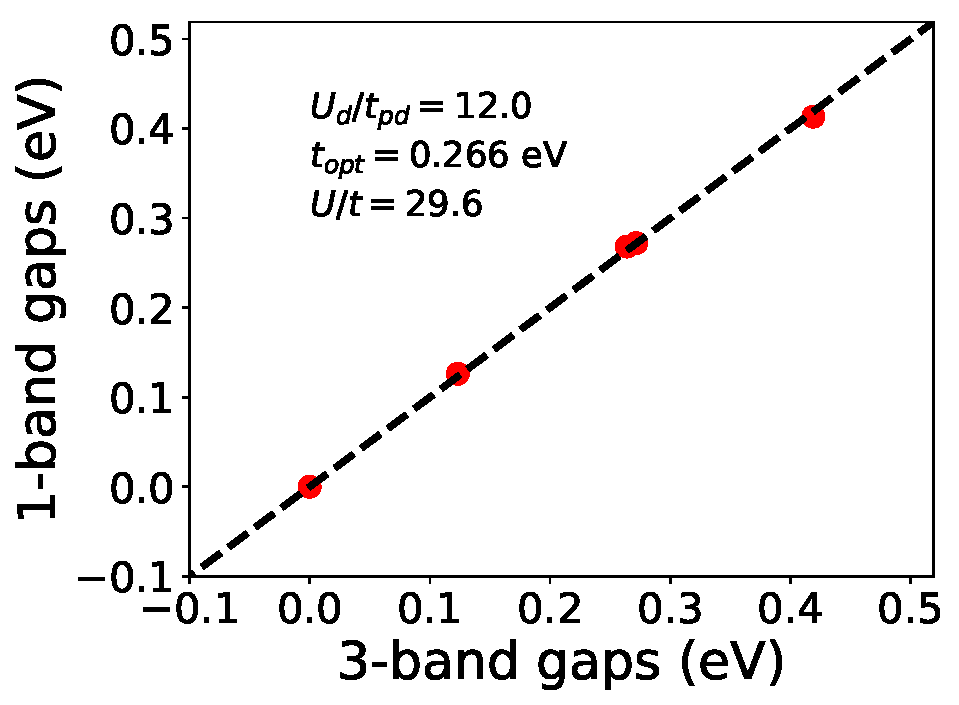
\includegraphics[width=0.325\linewidth]{./Figures/Gap_1_band_3_band_ep_5_number_2.pdf}
\caption{Comparison for energy gaps between the 3-band and 1-band Hubbard models 
using the optimized values of $U/t$ and $t$, for different $U_{d}/t_{pd}$ for $\Delta/t_{pd}=3$ (top row) 
and $\Delta/t_{pd}=5$ (bottom row)}
\label{fig:energyfit} 
\end{figure}	

Downfolding enables reduction of the size of the effective Hilbert space; allowing 
simulations of bigger unit cells to be carried out. To show that this actually works well in practice for the 3-band case, 
we consider the $2\sqrt{2} \times 2 \sqrt{2}$ square unit cell, comprising of 8 copper and 16 oxygen orbitals. 
For the test cases presented in Fig.~\ref{fig:energyfit}, we performed an exact diagonalization 
(or full configuration interaction) calculation at half filling, the Hilbert space comprises of 112911876 basis states. 
Roughly 200 Lanczos iterations were carried out, enabling convergence of the lowest four energies. 
We compared the lowest gaps with the corresponding calculation on the single 
band model with the same square geometry, with a Hilbert space size of only 4900, 
using the downfolded parameters obtained from the smaller $2 \times 2$ cell. Our results are summarized 
in Table~\ref{tab:predictivity}

\begin{table}[ht]
\centering
\begin{tabular}{c|c|c|c||c|c||c|c||c|c}
\hline
$\Delta/t_{pd}$ & $U_d/t_{pd}$ & $t$ & $U/t$ & $G_{2-1,3}$ & $G_{2-1,1}$ & $G_{3-1,3}$ & $G_{3-1,1}$ & $G_{4-1,3}$ & $G_{4-1,1}$  \\
                &              & (eV)&       & (eV)        & (eV)        & (eV)        & (eV)        & (eV)        & (eV)         \\
\hline
\hline
3.0 & 4.0 & 0.29 & 8.8 & 0.0465 & 0.0474 & 0.1505 & 0.1529 & 0.2247 & 0.2244  \\ 
3.0 & 8.0 & 0.31 & 13.3 & 0.0524 & 0.0542 & 0.1682 & 0.1726 & 0.2063 & 0.2082  \\ 
3.0 & 12.0 & 0.32 & 16.0 & 0.052 & 0.0538 & 0.1658 & 0.1696 & 0.192 & 0.1936  \\ 
5.0 & 4.0 & 0.237 & 15.1 & 0.0395 & 0.0405 & 0.1256 & 0.1281 & 0.1466 & 0.1485  \\ 
5.0 & 8.0 & 0.254 & 23.8 & 0.0344 & 0.0352 & 0.107 & 0.1086 & 0.1142 & 0.1154  \\ 
5.0 & 12.0 & 0.266 & 29.6 & 0.031 & 0.0316 & 0.0956 & 0.0967 & 0.0998 & 0.1006  \\ 
\hline
\end{tabular}
\caption{Comparison of low energy gaps of the 8 unit cell ($2\sqrt{2} \times 2\sqrt{2}$) at half filling for the 
1-band Hubbard (Hilbert space 4900) and 3-band Hubbard (Hilbert space 112911876) 
models from exact diagonalizations, for six representative cases using $t_{pd}=1.3 $ eV. The notation $G_{i-j,m}$ 
has been used to indicate the gap (energy difference) between state $i$ and $j$ and $m=1,3$ is a label that 
refers to the 1- or 3-band models. 
The downfolded parameters ($t$ and $U/t$) 
for the 1-band model were those obtained from downfolding the 4 unit cell ($2\times2$) case.}
\label{tab:predictivity}
\end{table} 

\HJC{Once the predicitivity objective is achieved for the lowest eigenstates, discuss the 6 test cases with DMD. 
This gets the average parameters that best describes the energy window, not only the extrema}


